\chapter{Background}
\label{ch:2}
\bigskip
As we all know that in India the politics and the social media is a big thing for people to consider as an important part of life. But the problem is that some social media users does think of exploiting with the content either by downloading the image or video or recording on screen and uploading it to the social media platforms. Those new images might be very sensitive and controversial and that becomes viral and put bad impact on the society.

The integrity of data has become more and more important. Security breaches that have leaked passwords and user emails are commonplace and regularly appear in the news. When a system is hacked, the first issue that usually comes to mind is the compromise of confidentiality, specifically what confidential information is now in the hands of the adversary.
Another aspect, which is getting increasingly important, is to know the integrity of data, has anything been changed contextually in order to address the higher level question: \q{Can we trust that this data is the actual data?}.
The need to verify the integrity of the data varies between different organizations. For example, in health care, incorrect information could be life threatening, while in industries such as finance in authentic data could be associated with great cost. Social media platforms are presenting images on their platform with only a very low (almost nothing) level of verification, often next to paid content and advertising. Companies paying for distribution of content and advertising have an inherent interest to know that their content is being displayed reliably and in the case of advertisements that the content displayed next to their content is reliable, \textit{i.e.}, that it has not been compromised.
This thesis will investigate the possibility of verifying the integrity of image content using blockchains. The resulting system should be capable of being implemented on various platforms, such as social media platforms.

This chapter introduces the reader to all the relevant background knowledge needed to grasp all of this thesis.
Section \ref{sec:image} details what an image is generated and how it can be decoded.
In Section \ref{sec:blockchain} describes the intricacies of the main underlying concepts that comprises a blockchain.
The Section \ref{sec:mlearning} is a little introductory part of the new emarging technology Machine Learning where computers have programmed in such a way that they seems they are learning and adapting with the changes of the environment. We introduced it because we are gonna use this to compare images using their contexts.
Section \ref{sec:security} talks about the security of our system with regards to device to device communication.
Section \ref{sec:client} details the client framework and what components \& Application Programming Interfaces (APIs) will be used to create the prototype mobile or computer client.
Section \ref{sec:server} explains the front end development done for the web server, focusing mainly on the necessary JavaScript development.
Section \ref{sec:prevWorks} discusses related projects that have been done
both in academia and in the industry.
Lastly, Section \ref{sec:summary} summarizes the background information and lays a theoretical foundation for this thesis.

\section{Image}
\label{sec:image}
Image can be described what we see at a particular instance of time, as we can sense that we are in a 4 dimentional video space 3 D's for space (height, width, depth) and 1 D for time. Images that are captured in the digital camera (like an eye) by burning a integrated circuit chip portion called memory can be stored in different file formats for future use.

Image file formats are standardized means of organizing and storing digital images. Image files are composed of digital data in one of these formats that can be rasterized for use on a computer display or printer. An image file format may store data in uncompressed, compressed, or vector formats. Once rasterized (making a matrix of intensity vaues of pixel positions), an image becomes a grid of pixels, each of which has a number of bits to designate its color equal to the color depth of the device displaying it.

The size of raster image files is positively correlated with the number of pixels in the image and the color depth (bits per pixel). Images can be compressed in various ways, however. A compression algorithm stores either an exact representation or an approximation of the original image in a smaller number of bytes that can be expanded back to its uncompressed form with a corresponding decompression algorithm. Images with the same number of pixels and color depth can have very different compressed file size. Considering exactly the same compression, number of pixels, and color depth for two images, different graphical complexity of the original images may also result in very different file sizes after compression due to the nature of compression algorithms. With some compression formats, images that are less complex may result in smaller compressed file sizes. This characteristic sometimes results in a smaller file size for some lossless formats than lossy formats. For example, graphically simple images (\textit{i.e.} images with large continuous regions like line art or animation sequences) may be losslessly compressed into a GIF (Graphics Interchange Format) or PNG (Portable Network Graphics) format and result in a smaller file size than a lossy JPEG (Joint Photographic Experts Group) format. With vector images the file size increases only with the addition of more vectors.

There are two types of image file compression algorithms: lossless and lossy.
\textbf{Lossless compression} algorithms reduce file size while preserving a perfect copy of the original uncompressed image. Lossless compression generally, but not always, results in larger files than lossy compression. Lossless compression should be used to avoid accumulating stages of re-compression when editing images.
\textbf{Lossy compression} algorithms preserve a representation of the original uncompressed image that may appear to be a perfect copy, but it is not a perfect copy. Often lossy compression is able to achieve smaller file sizes than lossless compression. Most lossy compression algorithms allow for variable compression that trades image quality for file size.

\section{BlockChain}
\label{sec:blockchain}
% BlockChain %
A BlockChain or \textbf{\q{The Truth Machine}} ~\cite{the_truth_machine} can be broadly described as a peer-to-peer network of nodes that makes a collaborative effort in sensing certain specified chain of blocks of data around its periphery and thereby controls the surrounding environment.
Accrrding to Wikipedia~\cite{blockchain_wiki} a blockchain, originally block-chain, is a growing list of records, called blocks, which are linked using cryptography. Each block contains a cryptographic hash of the previous block, a timestamp, and transaction data (generally represented as a Merkle tree).
In BlockChains, each node consists of processing capability, it may contain multiple types of memory like program, data and memories, having a Web-Service transceiver, Client-side processors, and a power source. The nodes communicate with each other using web-services and self-organized.
There are certain nodes called miners that veryfies each transactions or entry of data in the chain and are the most reliable personnel in the network who always have the updated copy of blocks of data.

\begin{figure}
\begin{center}
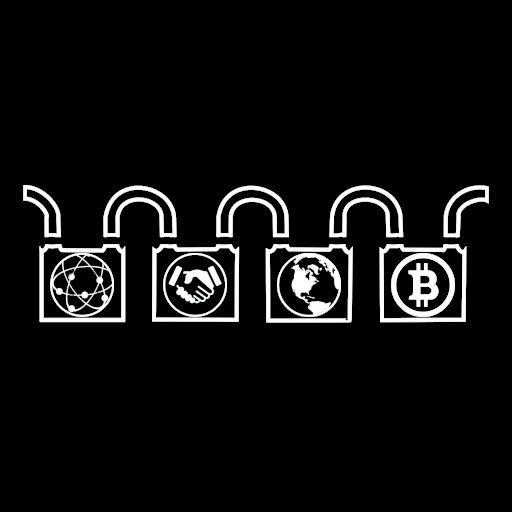
\includegraphics[width=0.5\textwidth]{./img_src/blockchain.jpg}
\end{center}
\caption{Overview of Block-Chain Technology (BCTs).}
\end{figure}

\subsection{What is Blockchain}
By definition blockchain is a decentralized computation and information sharing platform which enables multiple authoritative domains who do not trust each other to cooperate coordinate and collaborate in a rational decision making process.

The technology is particularly useful when multiple parties or individual they want to cooperate it with each other, and they want to come to a common platform to share the information among themselves.

Blockchain is that whenever we are talking about multiple authoritative domains.

This multiple authoritative domains they do not trust each other. So, this is an important aspect of blockchain that you can combine multiple authoritative domains who do not trust with each other and they can come to a common platform where they can cooperate, coordinate and collaborate in application development process at the business intelligence process.

Let's suppose in a blockchain platform Alice has her own copy of a document and Bob has his own copy of another document. So, the seperate copy belongs to Alice and Bob, and they can simultaneously write to their own document and here I have the network in between and the network has the task to ensure that the information consistencies maintained between the documents which Bob and Alice hold individually.

The advantage  is that that they do not need to rely on the internet or if a server crashes they do not depend on the server files.

So, by definition we can say that a blockchain is decentralized data based platform with strong consistency support.

\subsection{Blockchain Arcitecture}
So, the protocol for commitment means whenever someone is making a new transaction, during that time you need to ensure that this particular transaction if it is valid, it will get committed to the existing public ledger or the existing blockchain, otherwise that entry will not be there in the blockchain. So, there should be a mechanism for validity checking of every upcoming transactions from the clients and then based on that validity checking you will be able to either accept the transaction and include it in the existing blockchain or you can delete the transaction or discard the transaction.

The second requirements is a consensus. Consensus is an important aspect in the in the context of blockchain. So, in case of blockchain as we have discussed that everyone has a 
local copy of the information available to every individual parties and there is no such central platform like a bank which will maintain the consistency of the transactions or 
the consistency of the information. So, that is why the consensus mechanism ensures that whatever local copy every individual party has they are consistent with each other that 
everyone has the most updated copy, and a copy, that the individuals have, are identical or similar to each other. 

The third important aspect is the security. That means, the data that one is inserting in a public ledger or inside the blockchain, now because this blockchain is distributed to individual parties everyone is maintaining their local copy of the blockchain. So, that person may change something in that local copy and broadcast that saying that \q{see this is the updated information}.

Fourth aspects is the privacy and authenticity. The data or the transactions which is their inside the blockchain it belong to various clients. So, it is coming from various clients and you are putting that information inside the blockchain and a copy of the blockchain is available to every parties and that is why the privacy and authenticity of the information needs to be ensured.

Some of the underlying concepts of the BlockChain especially BitCoin (the most popular implementation of BlockChain) and some other important technology are briefed.

\subsection{Types}
There are two types of blockchain,

\subsubsection{Permissionless BlockChain}
Permissionless or Public blockchain networks power up most of the market's digital currencies. They allow every user to create a personal address and begin interacting with the network, by submitting transactions, and hence adding entries to the ledger. Additionally, all parties have the choice of running a node on the system, or employing the mining protocols to help verify transactions.

Additionally, for digital currencies such as Ethereum, the blockchain network also supports smart contracts, which are automated transactions that self-execute when certain criteria are met. As Ethereum also employs a permisionless blockchain, anyone can develop and add smart contracts onto the network, with no limitation imposed by the developers. Apart from allowing anyone to get involved on the network, there are few more characteristics associated with the permisionless model. These are:

\begin{itemize}
\item \textbf{Decentralization:} No central entity has the authority to edit the ledger, shut down the network, or change its protocols.
\item \textbf{Digital assets:} The presence of a financial system on the network.
\item \textbf{Anonymity:} It do not require users to submit personal information prior to being able to create an address, or submit transactions. However, in certain cases, personal information is required for legal purposes
\item \textbf{Transparency:} It needs to freely give users access to all information apart from the private keys from addresses, to how transactions are processed into blocks, and the freedom to see all transactions processed by the network.
\end{itemize}

\subsubsection{Permissioned BlockChain}
Permissioned or Private blockchain closed ecosystems, where users are not freely able to join the network, see the recorded history, or issue transactions of their own. Permissioned blockchains are preferred by centralized organizations, which leverage the power of the network for their own, internal business operations. Company consortiums are also likely to employ private blockchains to securely record transactions, and exchange information between one another.

\subsection{Peer-to-Peer Network}
This is the internet protocol that connects different logged in users as a node which is having some computation power. The users who are only uploading and verifying may have computer or smartphone, but the verifiers or the miners must have to work on computer with sufficient amount of computation power.

\begin{tikzpicture}[]
\node(node1)[node] {node1};
\node (pl1) [pl, left of=node1, xshift=-0.1cm] {};
\node(node2)[node, right of=node1, xshift=5cm] {node2};
\node (pl2) [pl, right of=node2, xshift=0.1cm] {};
\node(node3)[node, below of=node1, yshift=-3cm] {node3};
\node (pl3) [pl, left of=node3, xshift=-0.1cm] {};
\node(node4)[node, below of=node2, yshift=-3cm] {node4};
\node (pl4) [pl, right of=node4, xshift=0.1cm] {};
\node(node5)[node, right of=node1, xshift=2cm,yshift=2cm] {node5};
\node (pl5) [pl, above of=node5, yshift=0.3cm] {};
\node(node6)[node, right of=node3, xshift=2cm,yshift=-2cm] {node6};
\node (pl6) [pl, below of=node6, yshift=-0.3cm] {};

\draw[<->, thick] (node1) -- (node2);
\draw[<->, thick] (node1) -- (node3);
\draw[<->, thick] (node1) -- (node4);
\draw[<->, thick] (node1) -- (node5);
\draw[<->, thick] (node1) -- (node6);
\draw[<->, thick] (node2) -- (node3);
\draw[<->, thick] (node2) -- (node4);
\draw[<->, thick] (node2) -- (node5);
\draw[<->, thick] (node2) -- (node6);
\draw[<->, thick] (node3) -- (node4);
\draw[<->, thick] (node3) -- (node5);
\draw[<->, thick] (node3) -- (node6);
\draw[<->, thick] (node4) -- (node5);
\draw[<->, thick] (node4) -- (node6);
\draw[<->, thick] (node5) -- (node6);
\end{tikzpicture}


\subsection{Transactions}
Everything in crypto-currency comes under transactions, i.e. someone is sending some amount of money to someone else at some time. So a basic or overall transaction data can be structured as,

\fbox{\colorbox{lightgray}{\parbox[b][4cm][c]{0.50\linewidth}{
\textbf{\texttt{\noindent Transaction :: \{\\
\hspace*{1cm} \textless Transaction\_id\textgreater,\\
\hspace*{1cm} \textless TimeStamp\textgreater,\\
\hspace*{1cm} \textless Sender\_Id\textgreater,\\
\hspace*{1cm} \textless Receiver\_Id\textgreater,\\
\hspace*{1cm} \textless Amount\_Unit\textgreater\\
\noindent \}}}
}}}

This transaction details is send to every peer to verify. If they heard already about it, it is true, or it is false (same as women's un-manipulated gossip in village). If more than 50\% population declare it true, then it is allowed to be in the Public Ledger.

\subsection{Public Ledger}
This is the publicly shared record of transactions kept as a list of blocks. At a particular point of time everybody (every node), who are connected to the network, should have a same copy of ledger in their own devices of what server has. Whenever a new person logs into the network aotomatically the server forces to update the ledger to the person's device. So basically the ledger is the chain file.

\subsection{Chain of Blocks}
It means list of blocks of data having some common part with previous and next block. This is like Single-way linked-list(every node consists of data and program memory address to the next node). Every block contains a number of transactions and many more things.

\fbox{\colorbox{lightgray}{\parbox[b][6cm][c]{0.75\linewidth}{
\textbf{\texttt{\noindent Block :: \{\\
\hspace*{1cm} \textless Block\_Id\textgreater,\\
\hspace*{1cm} \textless TimeStamp\textgreater,\\
\hspace*{1cm} \textless Merkle\_Root\textgreater,\\
\hspace*{1cm} \textless Verifier\_Id\textgreater,\\
\hspace*{1cm} \textless Nonce\_Value\textgreater,\\
\hspace*{1cm} \textless Previous\_Hash\textgreater,\\
\hspace*{1cm} \textless Current\_Hash\textgreater,\\
\hspace*{1cm} \textless Data :: ANumberOfTransactions\textgreater\\
\noindent \}}}
}}}

So it is kind of backword linked-list which is propagating by having the previous block's kind of identity (because there is a mild chance of collision i.e. multiple values' hashes are same) hash.

\subsection{Timestamp}
The time means absolute global date-time in the format: 

\fbox{\colorbox{lightgray}{\parbox[b][2cm][c]{\linewidth}{
\textbf{\texttt{\noindent TimeStamp :: String (
\textless day\_of\_week\_code :: ddd\textgreater,
\textless month\_code :: mmm\textgreater,
\textless day\_of\_month :: dd\textgreater,
\textless year :: yyyy\textgreater,
\textless time :: hh:mm:ss\textgreater,
\textless Distance from Mean-TimeLine :: GMT+hhmm\textgreater,
\textless Time Zone :: Country\_Name Standard Time\textgreater
\noindent )}}
}}}

Example: \textbf{\q{Sat May 25 2019 20:45:04 GMT+0530 (India Standard Time)}}. The timestamp is one of the most needed to prove it later for verification of the record. It is used to create the current block's hash.

\subsection{Hash}
The job of a hash algorithm is to map any size of domain to a particular size of range. SHA-256 is one of the most popular hash algorithms which takes any length input and returns 256 bit output. All input/output operations can be transferred into strings.

\subsection{Merkle Root Hash}
Merkle tree is a complete binary tree which has the hash values of transaction data as leaf nodes. The tree propagation occures from leaves to root as tournament tree form. For any point,

			parent hash = hash(child-1 hash + child-2 hash);

A little change in any data of any transaction will change the merkle root, and thus the block's hash and the complete chain. Because it is used to create the current block's hash.

\begin{tikzpicture}[]
\node (root) [process] {H\_r = hash(H\_0 + H\_1)};
\node (child1) [process, below of=root, xshift=-4cm, yshift=-2cm]{H\_0 = hash(H\_0-0 + H\_0-1)};
\node (child2) [process, below of=root, xshift=4cm, yshift=-2cm]{H\_1 = hash(H\_1-0 + H\_1-1)};
\node (child3) [process, below of=child1, xshift=-2cm, yshift=-2cm]{hash(TxD\_0)};
\node (child4) [process, below of=child1, xshift=2cm, yshift=-2cm]{hash(TxD\_1)};
\node (child5) [process, below of=child2, xshift=-2cm, yshift=-2cm]{hash(TxD\_2)};
\node (child6) [process, below of=child2, xshift=2cm, yshift=-2cm]{hash(TxD\_3)};

\node (txd0) [process, below of=child3, yshift=-2cm] {TxD\_0};
\node (txd1) [process, below of=child4, yshift=-2cm] {TxD\_1};
\node (txd2) [process, below of=child5, yshift=-2cm] {TxD\_2};
\node (txd3) [process, below of=child6, yshift=-2cm] {TxD\_3};

\draw [arrow] (child1) -- (root);
\draw [arrow] (child2) -- (root);
\draw [arrow] (child3) -- (child1);
\draw [arrow] (child4) -- (child1);
\draw [arrow] (child5) -- (child2);
\draw [arrow] (child6) -- (child2);
\end{tikzpicture}


\subsection{Previous Hash}
The previous block's hash. It is required to maintain the chain system because we can not create the next address and we don't know when it would be created, so it is better to store what we already have. It is used to create the current block's hash.

\subsection{Nonce}
It is the quantity of computation power used to solve a mathematical problem which is not so hard but not so easy either. Too easy solution will be easy to break and too hard solution will take so long time to create a block that the adversary with huge computation power have a chance to alter the data before creating and verifying a block. Rather a medium hard problem will be better. It is used to create the current block's hash.

This is to show the verifiers that the block creator have spent sufficient amount of computation power before creating the block and also to delay the process a little bit and this is called POW (Proof of Work). In bitcoin the problem is to find the first hash of given values which is having 'd' number of leading 'zero's where the 'd' represents the difficulty of the problem i.e. the more 'd' gets it will take longer to calculate. Typical value of 'd' is 32 bits and average delay for the whole block addition (create, verify then add) is about 10 minutes.

\subsection{Consensus Mechanism}
It is the contract or the protocol by which the blocks are verified and the winning blocks are added to everyone's ledger as well as the central server. The actual consensus algorithm is not published for security reasons. But by possible ways or reverse eengineering people have created  different models. Some of those models are:

\begin{figure}
\begin{center}
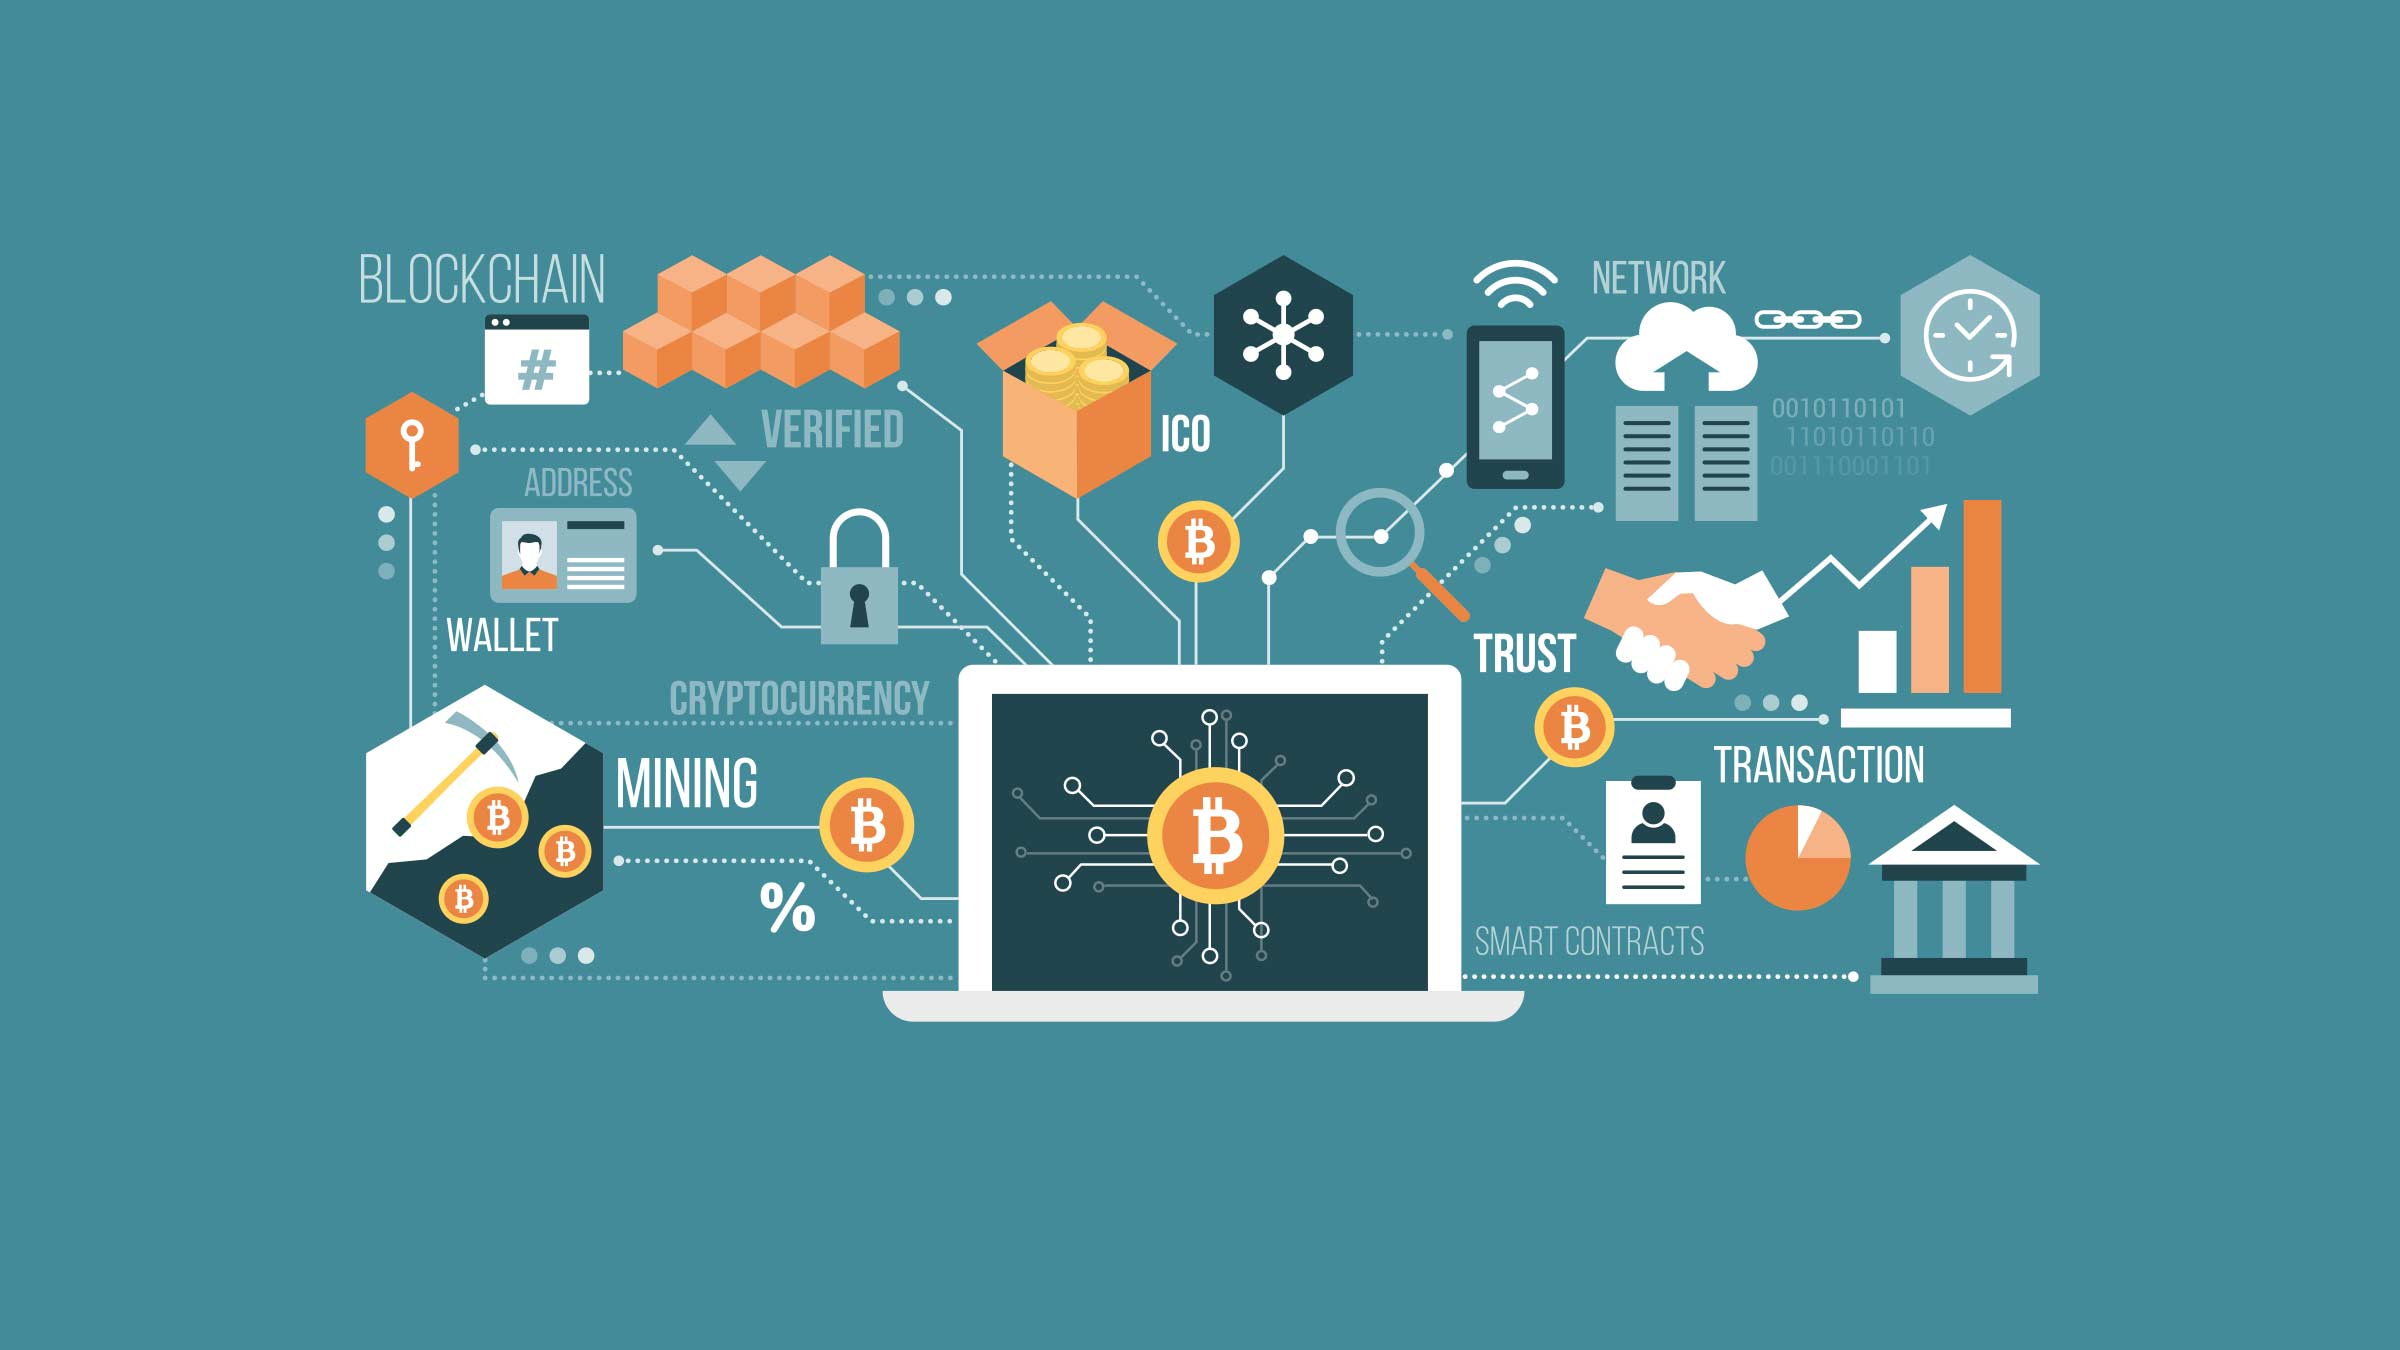
\includegraphics[width=0.75\textwidth]{./img_src/bitcoin.jpg}
\end{center}
\caption{Overview of BitCoin Technology (BCTs).}
\end{figure}

\begin{enumerate}
\item Probable bitcoin consensus mechanism
\item Paxos (Part-Time Parliament) consensus mechanism~\cite{paxos_made_easy, paxos_made_practical}
\item Raft consensus mechanism~\cite{raft_extd}
\end{enumerate}

Bitcoins one is probably the simplest one, but having bugs. The Paxos allows different types of sources and faults to come, it learns and fixes it. Raft does not allow any fault to happen.

The basic overall way in which consensus happen in bitcoin might be the following,

\begin{enumerate}
\item The transaction comes to server from client nodes;
\item Server stores that in file system database as unverified transaction;
\item At the point of interval of 10 minutes server broadcasts it to the miners network i.e. to every miner;
\item Each miner individually verifies and adds correct transaction in a block. Each node holds its block creation and validates the new block as soon as it gets new block from network. Who's block is valid and introduced first to network will be added to everyone's chain and they will start making new block on top of it. Sometimes forks might be created for the networking distance between distant nodes, at that moment conflict will come. If a new introduced block's previous hash does not match with the last block's current hash the node requests to the network to get the missing blocks one by one until the blocks match, it validates it, delete the wrong blocks (make them orphan) and add missing blocks to own chain to resolve fork and maintain longest updated chain. So it is a race between miner nodes.
\item Server gets a copy from miners group and updates own copy and delete the added tansactions from file system.
\end{enumerate}

\subsection{Applications of BCTs}
Block-Chain Technology provides one major advantage over conventional centralized database system: immunity from unexpected data changes or Hacks, which gives rise to numerous applications. Some of them include

\begin{itemize}
\item Crypto-currency: Creating and transferring digital money, Data Mining.
\item Military applications: Secure and verified records of Every Military Events and documents.
\item Structural health Monitoring
\item e-Biding Systems
\item Election System or e-Voting Systems
\item Selling Records and other Commercial Applications
\item Music Copyright Verification System
\item Integrity Analysis of Media Files
\end{itemize}

\subsection{Application}
Some of the commercial applications built on blockchain technology are as follows,

\subsubsection{BitCoin}
One year after creating protocols of BlockChian for cryptocurrency, Satoshi Nakamoto in 2009 released the first source code for BitCoin (BTC) application. Bitcoin has since grown rapidly to a market footprint of around 39 billion U.S. dollars (as of 12 Jul 2017). BTC is a decentralized cryptocurrency using a permissionless blockchain that every user has the ability to download and thereby check. The users of the network use their personal computational power to verify transactions through hashes, i.e., mining. The total computational power of the Bitcoin network is estimated to be more than 256 times the power of the world's 500 top supercomputers.
Site: \href{https://bitcoin.org/}{BitCoin}.

\subsubsection{HyperLedger}
Hyperledger is a project under the Linux Foundation which seeks to provide a unified blockchain architecture for industrial applications. Hyperledger is a collaboration of more than 100 organizations focused on banking, supply chain, and other transaction networks. It uses BFT system to reach consensus by fewer number of nodes.
\href{https://www.hyperledger.org/}{HyperLedger}

\subsubsection{Ethereum}
It is a permissionless blockchain made as a smart contracts platform run by Ether (ETH). The verification is done through the peer to peer network which constitutes Ethereum together with ETH which fuels the network, the consensus algorithm to share the state of the network, and the Turing complete scripting language which enables users to write complex scripts (smart contracts). It is the consensus engine which sets the speed of the Ethereum network by updating the state of the network at specific time intervals (shorter than for the Bitcoin network). The Ethereum network is fueled by gas which is a unit connected to ETH which is used to pay for the storage and computations an application (smart contract) needs.
\href{https://www.ethereum.org/}{Ethereum}

Solidity is a programing language build specifically to target the Ethereum virtual Machine (EVM) which in turn is the protocol to access the blockchain. Solidity has a syntax similar to JavaScript and is the language in which many smart contracts are written. The smart contracts are then compiled into bytecode and fed into to EVM and thus they can operate on the blockchain. In Ethereum are every transaction and smart contract is saved on the blockchain. The blockchain is in turn distributed and the states are handled by the consensus algorithm.
\href{https://solidity.readthedocs.io/en/v0.5.7/}{Solidity}

\subsubsection{Tendermint}
Tendermint is not a blockchain in itself but rather a general purpose blockchain consensus engine with a consensus layer for blockchaining. Tendermint can be used as a replacement for the consensus engines of other blockchains. It runs BFT algorithm.
\href{https://tendermint.com/}{Tendermint}

\subsubsection{Eris:db}
Eris:db is a controllable (permissible), smart contract-enabled, PoS based blockchain design with the PoS based on Tendermint. Eris:db is an application layer for blockchain applications. Eris is the backbone for deploying and interacting with the application logic.
\href{https://github.com/vulcanize/eris-db}{Eris:db}

\subsubsection{Cumulus}
Cumulus is a blockchain solution developed by Ericsson. Cumulus builds on and works with the Ethereum Virtual Machine (EVM) but separates the consensus algorithm and the blockchain from the EVM. Cumulus works similar to Ethereum; however, it is a private blockchain which means it does not run on gas.
\href{https://github.com/ubclaunchpad/cumulus}{Cumulus}

\subsection{Comparison}
There are a number of blockchain solutions to choose from, some of the most important ones are described in the previous subsections. For this thesis we will use a hybrid one, that supplies our requirements or logical proposal.

\begin{center}
\begin{tabular}{|c|c|c|c|c|c|}
\hline
\textbf{Name} & \textbf{Distribution} & \textbf{Transactions/second} & \textbf{Consensus Algorithm} \\
\hline
\textbf{Hyperledger} & Private & 10k & BFT \\
\hline
\textbf{Eris:db} & Private & 10k & Tendermint(PoS) \\
\hline
\textbf{Ethereum} & Public & 20 & PoS \\
\hline
\textbf{Tendermint} & Private & 10k & Tendermint BFT \\
\hline
\textbf{Bitcoin} & Public & 7 & PoW \\
\hline
\textbf{Cumulus} & Private & (untested) & (unknown) \\
\hline
\end{tabular}
\end{center}

\subsection{Security and Integrity in BCTs}
As the data is not sitting on a single data server so there is no security issue for Server Hacking. And also the hash-Chain with Cryptography makes it near to impossible to figure out or change previous data block in the blockchain. Before adding any data block with the help of consensus mechanism the blocks are verified with the digital signature of the node and some solution of nonce (the number of times the cllient application required to calculate the mathematical problem) and various other meta data.
As in some interval the system is refreshing itself, if some error seems to be occured, it backs up itself by contacting the miners (the trusted nodes), compare their files and back up with the valid one. So no integrity problem is there, unless and until the internet works fine.


\section{Machine Learning}
\label{sec:mlearning}
% Machine Learning
A machine is said to be learning from past Experiences(data feed in) with respect to some class of Tasks, if it's Performance in a given Task improves with the Experience.

According to a famous person, Machine Learning is a system that can learn from example through self-improvement and without being explicitly coded by programmer. The breakthrough comes with the idea that a machine can singularly learn from the data (\textit{i.e.} media database of real life objects, numbers dataset from algorithms, face images, job dtabase) to produce accurate results.

Machine learning combines data with statistical tools to predict an output. This output is then used by corporate to makes actionable insights. Machine learning is closely related to data mining and Bayesian predictive modeling. The machine receives data as input, use an algorithm to formulate answers.

A typical machine learning tasks are to provide a recommendation. For those who have a Netflix account, all recommendations of movies or series are based on the user's historical data. Tech companies are using unsupervised learning to improve the user experience with personalizing recommendation.

\subsection{Machine Learning vs. Traditional Programming}
Traditional programming differs significantly from machine learning. In traditional programming, a programmer code all the rules in consultation with an expert in the industry for which software is being developed. Each rule is based on a logical foundation; the machine will execute an output following the logical statement. When the system grows complex, more rules need to be written. It can quickly become unsustainable to maintain.

Machine learning is supposed to overcome this issue. The machine learns how the input and output data are correlated and it writes a rule. The programmers do not need to write new rules each time there is new data. The algorithms adapt in response to new data and experiences to improve efficacy over time.

\subsection{How does Machine learning work}
Machine learning is the virtual brain where all the learning takes place. The way the machine learns is similar to the human being. Humans learn from experience. The more we know, the more easily we can predict. By analogy, when we face an unknown situation, the likelihood of success is lower than the known situation. Machines are trained the same. To make an accurate prediction, the machine sees an example. When we give the machine a similar example, it can figure out the outcome. However, like a human, if its feed a previously unseen example, the machine has difficulties to predict.

The core objective of machine learning is the learning and inference. First of all, the machine learns through the discovery of patterns. This discovery is made thanks to the data. One crucial part of the data scientist is to choose carefully which data to provide to the machine. The list of attributes used to solve a problem is called a feature vector. You can think of a feature vector as a subset of data that is used to tackle a problem.

The machine uses some fancy algorithms to simplify the reality and transform this discovery into a model. Therefore, the learning stage is used to describe the data and summarize it into a model.

For instance, the machine is trying to understand the relationship between the wage of an individual and the likelihood to go to a fancy restaurant. It turns out the machine finds a positive relationship between wage and going to a high-end restaurant: This is the model

\subsubsection{Inferring}
When the model is built, it is possible to test how powerful it is on never-seen-before data. The new data are transformed into a features vector, go through the model and give a prediction. This is all the beautiful part of machine learning. There is no need to update the rules or train again the model. You can use the model previously trained to make inference on new data.

The life of Machine Learning programs is straightforward and can be summarized in the following points:
\begin{enumerate}
\item Define a question
\item Collect data
\item Visualize data
\item Train algorithm
\item Test the Algorithm
\item Collect feedback
\item Refine the algorithm
\item Loop 4-7 until the results are satisfying
\item Use the model to make a prediction
\end{enumerate}

There are two main types of Learning,
\subsubsection{Supervised learning}
An algorithm uses training data and feedback from humans to learn the relationship of given inputs to a given output. For instance, a practitioner can use marketing expense and weather forecast as input data to predict the sales of cans.

You can use supervised learning when the output data is known. The algorithm will predict new data.

There are two categories of supervised learning:
\paragraph{Classification}
Imagine you want to predict the gender of a customer for a commercial. You will start gathering data on the height, weight, job, salary, purchasing basket, etc. from your customer database. You know the gender of each of your customer, it can only be male or female. The objective of the classifier will be to assign a probability of being a male or a female (\textit{i.e.}, the label) based on the information (\textit{i.e.}, features you have collected). When the model learned how to recognize male or female, you can use new data to make a prediction. For instance, you just got new information from an unknown customer, and you want to know if it is a male or female. If the classifier predicts male = 70\%, it means the algorithm is sure at 70\% that this customer is a male, and 30\% it is a female.

The label can be of two or more classes. The above example has only two classes, but if a classifier needs to predict object, it has dozens of classes (\textit{e.g.} glass, table, shoes, etc. each object represents a class).

\paragraph{Regression}
When the output is a continuous value, the task is a regression. For instance, a financial analyst may need to forecast the value of a stock based on a range of feature like equity, previous stock performances, macroeconomics index. The system will be trained to estimate the price of the stocks with the lowest possible error.

\subsubsection{Unsupervised learning}
In unsupervised learning, an algorithm explores input data without being given an explicit output variable (\textit{e.g.} explores customer demographic data to identify patterns)

You can use it when you do not know how to classify the data, and you want the algorithm to find patterns and classify the data for you

Challenges and Limitations of Machine learning
The primary challenge of machine learning is the lack of data or the diversity in the dataset. A machine cannot learn if there is no data available. Besides, a dataset with a lack of diversity gives the machine a hard time. A machine needs to have heterogeneity to learn meaningful insight. It is rare that an algorithm can extract information when there are no or few variations. It is recommended to have at least 20 observations per group to help the machine learn. This constraint leads to poor evaluation and prediction.

\subsection{Application}
There are plenty of application fields where ML is being used for better performance,
\subsubsection{Augmentation}
Machine learning, which assists humans with their day-to-day tasks, personally or commercially without having complete control of the output. Such machine learning is used in different ways such as Virtual Assistant, Data analysis, software solutions. The primary user is to reduce errors due to human bias.
\subsubsection{Automation}
Machine learning, which works entirely autonomously in any field without the need for any human intervention. For example, robots performing the essential process steps in manufacturing plants.
\subsubsection{Finance Industry}
Machine learning is growing in popularity in the finance industry. Banks are mainly using ML to find patterns inside the data but also to prevent fraud.
\subsubsection{Government organization}
The government makes use of ML to manage public safety and utilities. Take the example of China with the massive face recognition. The government uses Artificial intelligence to prevent jaywalker.
\subsubsection{Healthcare industry}
Healthcare was one of the first industry to use machine learning with image detection.
\subsubsection{Marketing}
Broad use of AI is done in marketing thanks to abundant access to data. Before the age of mass data, researchers develop advanced mathematical tools like Bayesian analysis to estimate the value of a customer. With the boom of data, marketing department relies on AI to optimize the customer relationship and marketing campaign.
\subsubsection{Supply Chain}
Machine learning gives terrific results for visual pattern recognition, opening up many potential applications in physical inspection and maintenance across the entire supply chain network.

Unsupervised learning can quickly search for comparable patterns in the diverse dataset. In turn, the machine can perform quality inspection throughout the logistics hub, shipment with damage and wear.

For instance, IBM's Watson platform can determine shipping container damage. Watson combines visual and systems-based data to track, report and make recommendations in real-time.

In past year stock manager relies extensively on the primary method to evaluate and forecast the inventory. When combining big data and machine learning, better forecasting techniques have been implemented (an improvement of 20 to 30 \% over traditional forecasting tools). In term of sales, it means an increase of 2 to 3 \% due to the potential reduction in inventory costs.

\paragraph{Google Car}
For example, everybody knows the Google car \textbf{Waymo}. The car is full of lasers on the roof which are telling it where it is regarding the surrounding area. It has radar in the front, which is informing the car of the speed and motion of all the cars around it. It uses all of that data to figure out not only how to drive the car but also to figure out and predict what potential drivers around the car are going to do. What's impressive is that the car is processing almost a gigabyte a second of data.


For our case we use logistic regression (discussed in Appendix app:4) and the algorithm is discussed in Proposal chapter \ref{ch:3}.


\section{Security}
\label{sec:security}
In this thesis project data integrity is of paramount importance. In order to be able to trust the data stored within the blockchain, a reliable secure connection is created between the application running on cleent's device and the computer that is computing the blockchain. User side application collects the data and creates the consecutive transaction which is to be sent between the device and the server where the blockchain computations are done, therefore it is impossible for a third party to know what the plaintext representation of the image is.
As a result encryption of this transaction might be of less importance. However, it is crucial for the system to know that the integrity of the hash is intact. The image captured and stored at a device can later be verified as to what is received by another device by using the blockchain.
An HTTP connection is used between the device and the server. The HTTP connection will in future implementation be replaced with a HTTPS connection to secure the communication.

\begin{figure}
\begin{center}
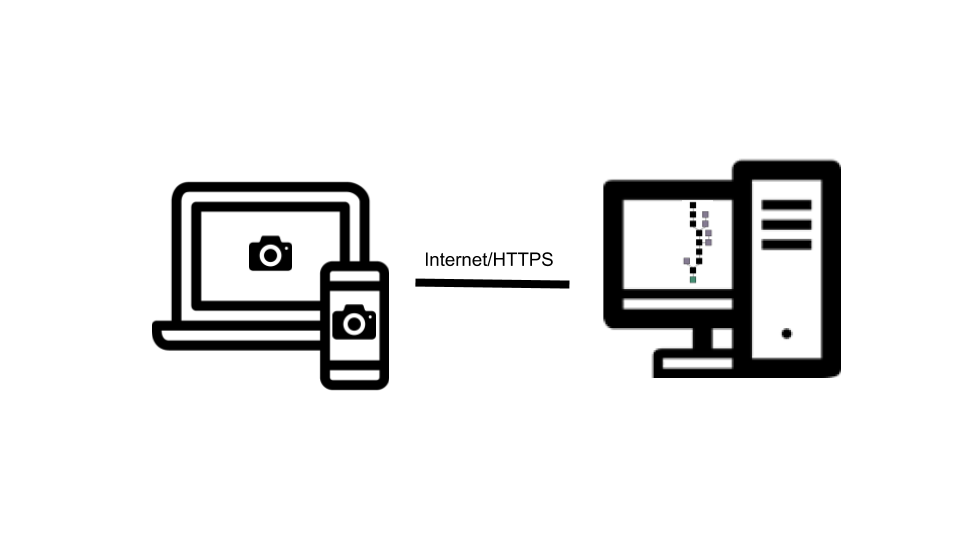
\includegraphics[width=\textwidth]{./img_src/client_server.png}
\end{center}
\label{fig_connClientServer}
\caption{A secure connection between Client and Server}
\end{figure}

\section{Client Side}
\label{sec:client}
A client may have a smartphone (of the brand Android, iPhone) or a computer (laptop or desktop). All of these devices comes with a default web-browsing tool like Google Chrome, Microsoft Edge, Mozilla Firefox or Mac Safari etc. All else a client needs an active reliable internet connection to communicate with sever. Moreover the miners have to have computers with better computation power. With the advancement of web programming languages with lots of APIs now it is very easy to capture an image or handle a local file and pass the data to the peer-to-peer network.

\subsection{JavaScript}
In this thesis, basic js is used as the run-time environment together with the inbuilt JS library installed on the browser. We are trying to use Node.js (also along with our code) that runs there servers, i.e., the consensus server. Note that all three servers run within the node.js environment on the computer hosting the web server and blockchain. JavaScript is the front end development language which realizes the functionality of the web page. JavaScript works together with PHP (HTML in it) and CSS in order to deliver a nice looking functional web page.

\section{Server Side}
\label{sec:server}
\subsubsection{PHP Server}
The Server side is made of PHP (HTML-5). In order to easy communicate with the blockchain from both the client device and the server running the verification client PHP APIs used over the HTTP protocol, usually to the server's TCP port 80. An apache server is basically a web server architecture which enables clients to make a request of servers. The HTTP protocol builds upon a request/response relationship between a client and a server and in this case used within the LAMPP architecture. In HTTP a string is sent to a specific port on the server with a specific method predefined by the HTTP standard. The most common methods are: GET, HEAD, POST, and PUT. The POST method is used by both the Android device and the web client of this thesis project to give both the ability to add and via the reply to this POST request to get information from the server. The communication between JS and PHP is done with XML-HTTP request with JSON byte stream. There is every type of handwriten PHP code to handle any type of request to Server.
\subsubsection{POST Method}
The POST method is a standard method in the HTTP protocol and gives the user the ability to add and receive data from the server. A HTTP transaction session is established through a TCP connection to a specific port on the server. After the TCP connection is established, of plain text HTTP message is sent to the other who either confirms the transaction or responds with an error message. It is in the body of this message that the response to the sender will be sent. Within the scope of this thesis the response will either be a boolean variable showing a successful transmission or a string of hashes requested from the blockchain.
\subsubsection{HTTPS}
Hypertext Transfer Protocol Secure (HTTPS) is an encrypted version of the HTTP protocol. HTTPS is usually used for sensitive information such as banking, private information, or classified information. HTTPS usually uses port 443 rather than HTTP port 80. In order for a user to be able to trust that a server is who it says that it issigned, third party certificates are used, usually in conjuction with the use of the Secure Socket Layer (SSL) as a secure transport protocol. A third party provides the server with a signed certificate which the user of the service verifies. Now that the user has verified the identity of the client and the server has verified the identity of the client - and encryption between the two parties may be set up. The security depends on that the certification chain work, that the user knows which server to use and that the user (client) notices when the certificate is incorrect or missing. Furthermore, in order to provide a high level of security the keys and the algorithms used need to be strong.

\section{Related Works}
\label{sec:prevWorks}
\subsection{Old possible works}
The process of image integrity checking is old job and many algorithms have been made. The following is the overview of them.
\begin{enumerate}
\item Store the real images in some database. Match the testing image with the existing one bit by bit.
\item Like in previous case, store it and check the new one's hash with the existing one's hash.
\item Searching the image in different databases using object detection and context similarity.
\item Every digital image is created in an electronic device which is having some unique property or signature in the world. The softwares that has created the image are designed in such a way that they put the digital signature in the metadata field of the image, let's say EXIF data for JPEG images. Any software that knows the byte signatures can detect the random image is original or not by checking the signature and named context that lies inside of the image file.
\item By checking the image context with reality or possiblity, some images can be checked.
\item An expert or hacker not only seeks for the context or visual similarity, but an expert knows that secret figures (WaterMarking) secret messages (Steganography) can be embedded in the image file, because the main image is a 2d matrix of intensity values (list of integers for BnW, RGBA, CMYK, or other) at different pixel positions.
\item The modern approach is to use deep neural network that learns and tries to detect image integrity in about 90\% efficiency and accuracy.
\item Image Forensics uses about all of the previous ones.
\end{enumerate}

\subsection{Related Work}
This section presents related work done both in the academic world and the industry.
\subsubsection{Academic}
Three different academic papers have been identified as relevant to this research. The following subsections highlight their main points and relevance to this thesis project.
\paragraph{Timestamping video footage in traffic incidents}
In ~\cite{gkb_bitcoin} Gipp, Krosti, and, Breitinger investigated the use of the Bitcoin network to timestamp a video feed from a smartphone camera placed in a car in the event of an accident.
\paragraph{Trusted Timestamping}
With regards to trusted timestamping two reports were identified: \q{Trusted Timestamping} ~\cite{gmg_bitcoin} and \q{Commitcoin} ~\cite{ce_commitcoin}. Both solutions leverage the time stamp made using the Bitcoin protocol when creating a transaction together with the carbon dating nature of the blockchain (i.e., one can tell the rough date of an entry by looking at the sequence of time stamps). These two solutions are slightly different in terms of their execution, but the basic theory of using the existing Bitcoin blockchain is the same.
\paragraph{Forensics Investigations of Multimedia Data}
In ~\cite{pt_forensics}, R. Poisel and S. Tjoa review the latest trends in forensic investigations of multimedia data, i.e. images, videos, and audio files. They describe different methods for determining what has been done to images and expose fabrications down to which details within a picture have been tampered with.
\paragraph{Digital Watermarking}
I. Echizen, et al. ~\cite{esytth_watermark} insert digital watermarks into video files to detect data tampering. They begin by breaking a video file into its composonents: the video, the audio, the timecodes, and the eader. The header is used together with the timecodes to separately watermark the audio and video.
\subsubsection{Industrial}
Three different industry solutions have been identified as being relevant. The following subsections highlight their main points and relevance to this thesis project.
\paragraph{Nexan - Assureon Archive Storage}
In Assureon Archive Storage ~\cite{n_assureon} fingerprints are created from the data in order to prove the integrity of files within a data archive system. The original files are stored on at least two different disks or at two different geographical locations.
\paragraph{Enigio - time:beat}
The product series \q{time:beat} ~\cite{asa_enigio} includes: time:shot, time:stamp, time:grab, and time:mail: by Enigio. It uses to archive time stamped fingerprints of integrity sensitive materials: email, pictures, documents, and websites in a permissioned blockchain controlled and owned by Enigio.
\paragraph{Ascribe}
Ascribe ~\cite{h_intellect} helps artists to create a digital copy of their work and time-stamp it in the Bitcoin blockchain. When a file is uploaded, Ascribe creates a digital certificate which can be traded, tracked, or loaned via the blockchain using SPOOL ~\cite{dt_spool}.

\subsection{Curent Works}:
\begin{enumerate}
\item There are plenty of image storing and searching by image in the websites. In the list \href{https://images.google.com/}{Google Image}, \href{https://www.yandex.com/images/}{Yandex Images} they use the image searching by name, context.
\item Some of them uses object detection \href{https://images.google.com/}{Google Images}, \href{https://www.imageidentify.com/}{Wolfram Images}.
\item Some website programs use reverse image search like \href{https://images.google.com/}{Google Images}, \href{https://tineye.com/}{Reverse Image Search}.
\item There are plenty of softwares like the photo eding softwares itself like Photoshop, GNU Image Manipulation Program, and other editors.
\item In ~\cite{img_cnn} they used CNN for image comparing and many other that can be mentioned for well known face recognition problem.
\item In ~\cite{adam_fabian} they used a mechanism for video integrity analysis.
\end{enumerate}

\section{Summary}
\label{sec:summary}
The different parts and aspects of the proof of concept prototype were broken down and analyzed. From the smallest components of the blockchain consensus algorithms, to which existing blockchain platform should be utilized. It also talked about the ways of communication between server and client.
